
\chapter{\uppercase{Computational Results}}

In this chapter, we compare results of the time-discretized HOLO method to IMC with
a source tilting algorithm for two test problems~\cite{jayenne}.  Also, we
briefly compare performance in Section~\ref{timing}.  For all IMC results, no
local, discrete diffusion acceleration methods for effective scattering
(e.g., those in~\cite{imd,ddmc}) are applied.  Additionally, we demonstrate
the efficiency advantage of ECMC in our HOLO algorithm by comparing the results
to the same HOLO algorithm if the ECMC algorithm is replaced with a standard
Monte Carlo (SMC) simulation.  Finally, we present results that demonstrate
preservation of the equilibrium diffusion limit and the discrete maximum
principle by the HOLO algorithm.  Some of the results in this section were published
previously in~\cite{bolding_nse}.  
For the results in this chapter, the lumping-equivalent discretization
discussed in Sec.~\ref{sec:ldfe_fixups} is used for cells where the solution for
$\phi^{n+1}$ becomes negative.  When negative intensities in the HO solution produce
non-physical consistency terms, S$_2$ equivalent terms are used for the LO solve as
discussed in Sec.~\ref{sec:ho_easyfix}.

A measure of variance in cell-averaged scalar intensities was
calculated to provide a quantitative measure of the statistical accuracy of different solution
methods.  To form sample standard deviations, twenty independent simulations for each
particular result were performed using unique random number generator seeds.
The variance of a particular cell-averaged $\phi(x)$ is 
\begin{equation} 
    S_i^2 =  \frac{20}{20-1} \sum_{l=1}^{20} \left(\overline{\phi_{i}} -
    \phi_{i}^l\right)^2,
\end{equation}
where $\phi_{i}^l$ is the cell-averaged scalar intensity for cell $i$ from the $l$-th of 20 independent simulations and
$\overline{\phi_{i}}$ is the corresponding sample mean from the 20 simulations. To
provide a normalized, spatially-integrated result, we form a norm over cells as 
\begin{equation}
    \ss = \left({\frac{\sum\limits_{i=1}^{N_c}
S_i^2}{\sum\limits_{i=1}^{N_c}\overline{\phi_{i}}^2}}\right)^{1/2},
\end{equation}
where $N_c$ is the number of spatial cells. 

We will also form a figure of merit (FOM) to demonstrate how statistical accuracy
scales with the number of histories performed.  Our FOM is defined as
\begin{equation}\label{eq:fom}
    \FOM = \frac{1}{N_{\text{tot}}\ss^2}
\end{equation}
where $N_{\text{tot}}$ is the total number of histories performed over the simulation.
A larger value of the FOM indicates that the method produced less variance in the
solution per history performed, for a given problem.  This form of the FOM
is typically chosen because the variance is expected to reduce inversely proportional
to $N_{\text{tot}}$, so for standard MC simulations the FOM becomes, on average, independent of
$N_{tot}$~\cite{shultis_mc}.  The FOM is not necessarily expected to be independent
of $N_{\text{tot}}$ for IMC or
our HOLO method due to correlation of the solution between time steps; additionally, ECMC
has correlations between batches.





\section{Marshak Wave}
\label{sec:marsh}

For the first problem, the radiation and material energies are initially in
equilibrium at $2.5\times 10^{-5}$ keV.   An isotropic incident intensity of 0.150 keV is applied
at $x=0$; the incident intensity on the right boundary is $2.5\times10^{-5}$ keV.
The material properties are $\rho = 1$ g cm$^{-3}$ and $c_v = 0.013784$ jks/keV-g. The
absorption cross section varies as $\sigma(T) = 0.001\;\rho\; T^{-3}$ (cm$^{-1}$), for $T$
in keV.
The simulation was advanced until $t=5$~sh~(1~sh~$\equiv$~10$^{-8}$~s) with a fixed time step size of 0.001 sh. For comparison purposes, we
have not used adaptive mesh
refinement, only performed one HOLO iteration per time
step, and use a fixed 3 HO batches with equal number of histories per batch. A
relative tolerance of $10^{-6}$ for the change in $\phi(x)$ and $T(x)$ was used for
the LO newton solver for all results. Radiation energy
distributions are plotted as an effective temperature given by
$T_r=(\phi/(ac))^{0.25}$.  The effective temperature represents the temperature of the
material, if the material and temperature were in equilibrium.  Cell-averaged quantities are plotted.
For this problem, when negative values for $\phi^{n+1,\pm}(x)$ were detected, the lumping-equivalent
discretization was used within those cells and that Newton step was repeated.
Non-physical angular consistency terms were replaced with S$_2$-equivalent terms.kFor
reference, the fix-up in Sec.~\ref{sec:ldfe_fixups} that strictly enforces the floor temperature and preserves half-range
balance produced similar accuracy and stably converged for this problem.
\begin{figure}[hp]
    \centering
\begin{subfigure}{0.7\textwidth}
  \centering
    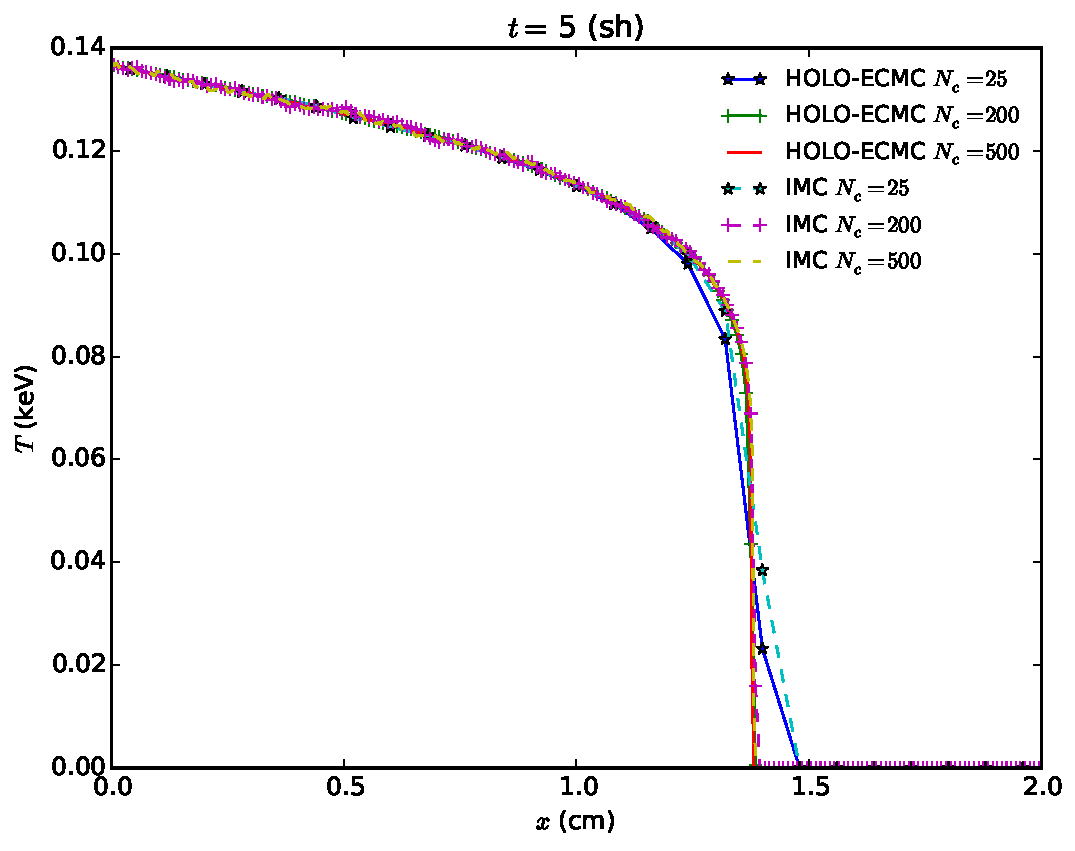
\includegraphics[width=0.99\linewidth]{marshak_mesh_conv.pdf}
    \caption{\label{marshak_mesh_conv} Convergence of IMC and HOLO-ECMC solutions.}
\end{subfigure}
\begin{subfigure}{0.7\textwidth}
  \centering
  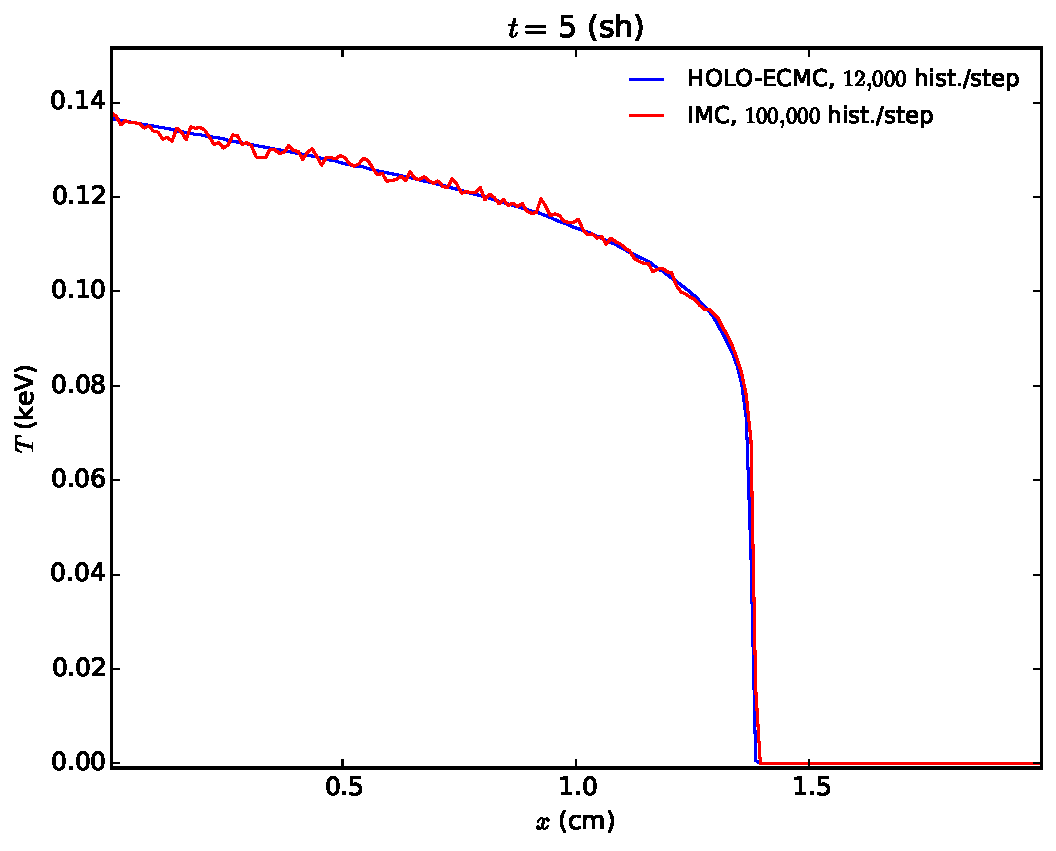
\includegraphics[width=0.99\linewidth]{marshak_200_compare.pdf}
  \caption{\label{marshak_200_compare}  Comparison of solutions for 200 spatial cells. }
\end{subfigure}
\caption{Comparison of radiation temperatures for Marshak wave problem at ${t=5}$ sh.}
\end{figure}

Figure~\ref{marshak_mesh_conv} on page~\pageref{marshak_mesh_conv} compares the cell-averaged radiation temperatures  for the
IMC and HOLO method with ECMC, for various number of spatial mesh cells $N_c$; we
have used HOLO-ECMC to denote our algorithm because later results will use different HO solvers.   For
all IMC calculations, $n=10^5$ histories per time step were used.  For the HOLO method, we have used
4 equal-sized cells in $\mu$ for the finite-element angular mesh used by the ECMC
solver.  The spatial grid is the same for the HO and LO solvers. For the cases
of $N_c=25$ and $N_c=200$, $4,000$ histories per batch ($n=12,000$ per time step)
were used.  For $N_c=500$, 16,000 histories per time step were used due to increased
number of space-angle cells that
need to be sampled. The IMC and HOLO solutions agree as the mesh is converged.  There is
similar agreement in the location of the wavefront due to the linear shape of the emission source over a cell.  The cells
nearest the wavefront required use of the lumping-equivalent discretization of the
radiation and
$S_2$ equivalent terms during the LO
solve, resulting in strictly positive cell-averaged quantities.  

Figure~\ref{marshak_200_compare} compares solutions
for the case of 200 cells.  For the IMC solution $10^5$ histories per time step were
simulated; for the HOLO method only $4,000$ histories per batch
(12,000 per time step) were simulated. There is significant statistical noise in the IMC solution
compared to the HOLO solution.  The HOLO solution visually demonstrates no
statistical noise.  Because the ECMC solve is only determining the change over the
time step, the statistical noise in the result is small relative to the magnitude of
$I^{n+1}$.  Also, the source sampling only places particles in cells where the residual is
large.  No particles are sampled in the equilibrium region out front of the wave.  Only a
few angular cells are necessary to accurately reproduce the mean intensity for this problem.

Table~\ref{marshak_var} compares $\ss$ and the FOM for IMC and the HOLO method, for different
numbers of histories per time step. The FOM results are normalized to the value for IMC with
$n=12,000$.  The HOLO method demonstrates less variance
for the same numbers of histories, producing FOM values that are two orders of magnitude greater than for IMC.  Where as the FOM remains relatively constant for
IMC, as $n$ is increased the FOM improves for the HOLO method.  This is a result of
each batch producing more statistically accurate estimates of the error $\epsilon$,
which results in an increased convergence rate of $\epsilon$ overall.  
\begin{table}[H]
\centering
\caption{\label{marshak_var} \textbf{Comparison of sample statistics for the Marshak Wave problem.   Simulation end time is $\mathbf{t=5}$ sh.}}
\vspace{-0.1in}
\begin{tabular}{|c|cc|cc|}\cline{2-5}
    \multicolumn{1}{c|}{}       & \multicolumn{2}{|c|}{\ss} &
    \multicolumn{2}{|c|}{\FOM} \\ \hline
hists./step   & IMC & HOLO-ECMC &  IMC & HOLO-ECMC   \\ \hline
   12,000	 & 3.40\%  & 0.28\% &  1    &  145      \\
  100,000    & 1.22\%  & 0.057\% & 0.93    &   422     \\ \hline
\end{tabular}
\end{table}



\section{Two Material Problem}
\label{sec:two}

This problem consists of an optically thin (left) and an optically thick (right) material region,
with temperature-independent cross sections.  The material properties are given in
Table~\ref{two_mat_props}.  Initially the radiation and material energies are in
equilibrium at a temperature of 0.05 keV.  An isotropic incident intensity of 0.500 keV
is applied at $x=0$ at $t=0$; the isotropic incident intensity on the right boundary is 0.05
keV.  The simulation end time is 5 sh. For all HOLO simulations, we have used 8
equal-sized mesh cells in $\mu$.  As for the Marshak problem, the cells nearest the wavefront required use of the lumping-equivalent discretization and
S$_2$-equivalent angular consistency terms during the LO solve.
\begin{table}[H]
        \caption{Material properties for two material problem\label{two_mat_props}}
\centering
        \begin{tabular}{|c|cc|}  \cline{2-3}
            \multicolumn{1}{c|}{}   & $x \in [0,0.5)$ cm & $x \in [0.5,1.0]$ cm   \\ \hline
            $\sigma_a$ (cm$^-1$)  & 0.2 & 2000 \\
            $\rho$ (g cm$^-3$) & 0.01 & 10.0 \\
            $c_v$ (jks/keV-g) & $0.1$ & $0.1$ \\ \hline
        \end{tabular}
\end{table}

Fig.~\ref{twomat_full} compares the HOLO and IMC radiation 
temperatures at the end of the simulation. The
IMC and HOLO results show good agreement
over the finer mesh.
On the coarse mesh ($N_c=20$), the LDFE representation of $T^4$ in the HOLO method predicts the location of the
wavefront more accurately than the IMC method with source tilting.

Fig.~\ref{compare_ho} demonstrates the benefit of ECMC as a HO solver compared to
standard MC.  The HOLO algorithm
with the ECMC HO solver (HOLO-ECMC) results
are for running 3 batches of 10,000 histories, per time step. The solution for the HOLO method with a standard MC solver as the HO solver
(HOLO-SMC) with standard source sampling uses 10$^5$ histories per time step. The HOLO-SMC solution demonstrates significant
statistical noise.  This noise is introduced into the LO solver by bad statistics in
computing the consistency terms. Also
plotted is an S$_2$ solution obtained with consistency terms that are equivalent
to S$_2$ and no HO correction.  The S$_2$ solution results in an artificially fast
wavefront, as expected, demonstrating the necessity of HO correction in this problem.

Table~\ref{twomat_var} compares the FOM and $\ss$ for IMC and the HOLO-ECMC method.  The FOM
values are normalized to the value for IMC with $n=30,000$.  The end time was reduced
to $2$ sh for these results to reduce computational times. The reduction in variance by
the HOLO method over IMC is substantial. The improvement of the FOM for the HOLO
method compared to IMC is greater than for the
Marshak wave problem.  This improvement is because the wave moves much slower in
right region of this problem, due to
the large, constant cross section.  Also, in the optically thin
region of the problem the solution quickly comes to equilibrium.  Thus, the ECMC
algorithm has to estimate a very small change in the intensity over a time step.  
\begin{figure}[H]
    \centering
\begin{subfigure}{0.65\textwidth}
    \centering
    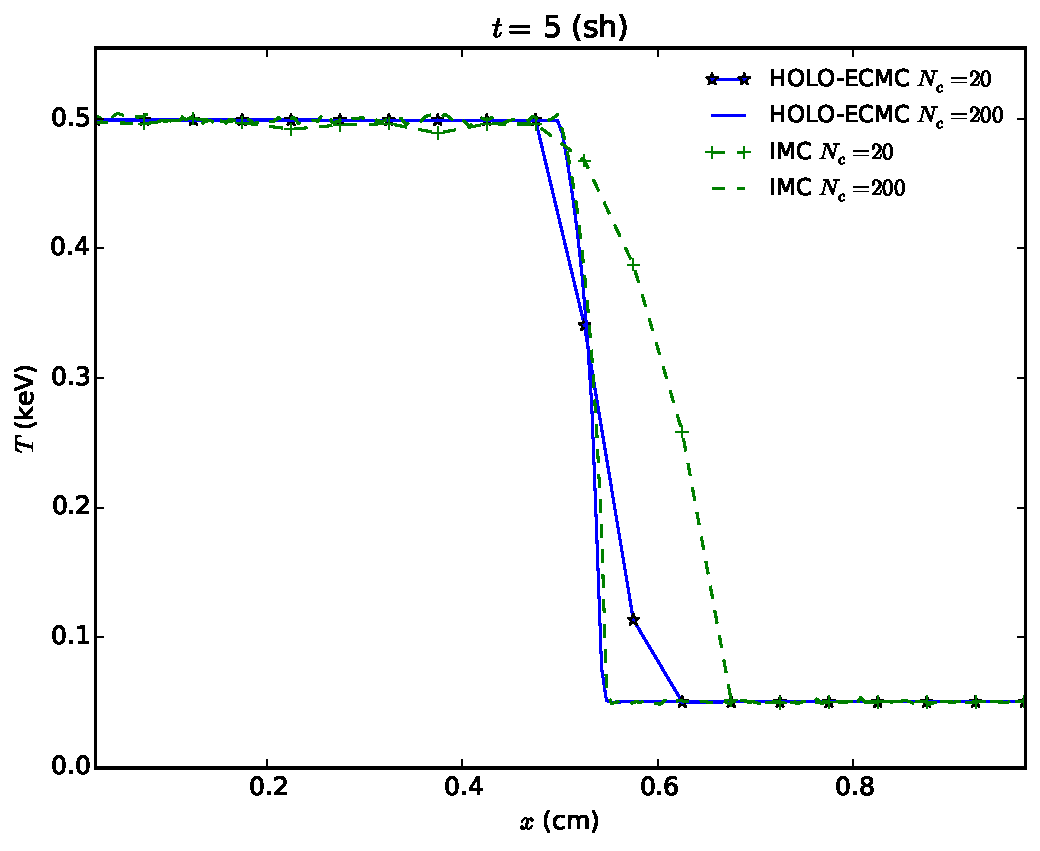
\includegraphics[width=0.99\textwidth]{two_mat_conv.pdf}
    \caption{Comparison of IMC and HOLO-ECMC.\label{twomat_full}}
\end{subfigure}    \begin{subfigure}{0.65\textwidth}
\centering
    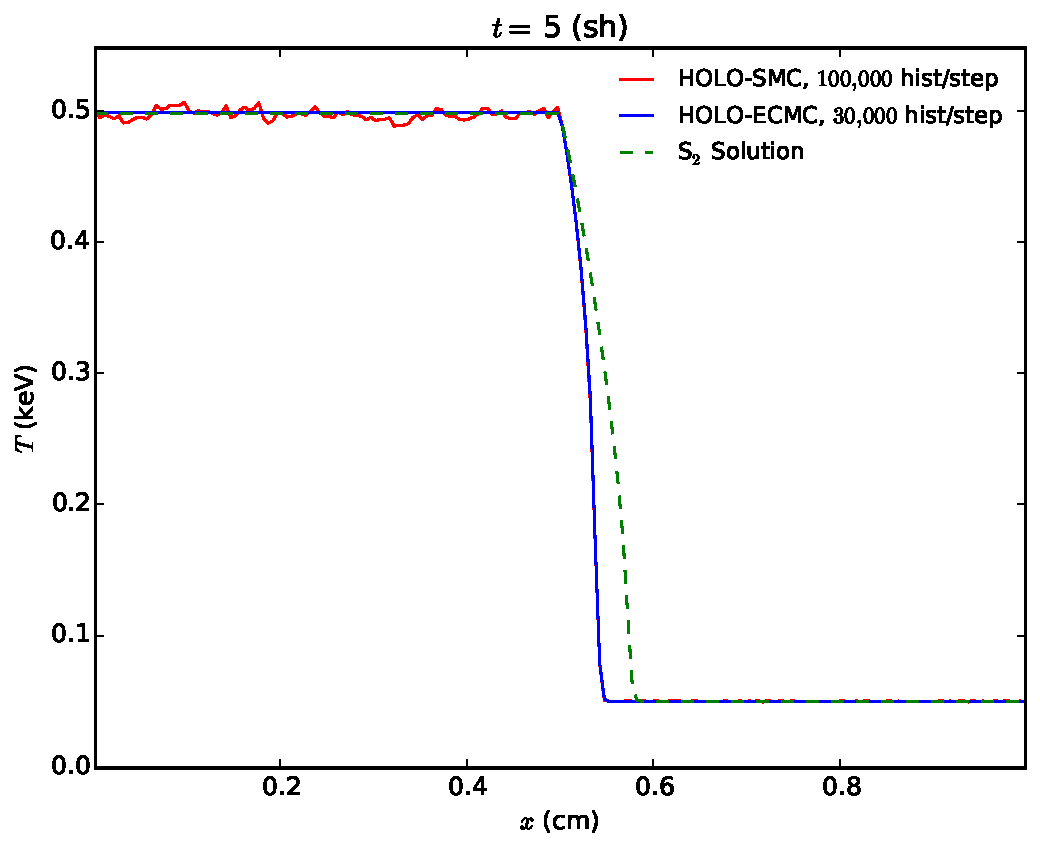
\includegraphics[width=0.99\textwidth]{two_mat_ho_compare.pdf}
    \caption{Comparison of SMC and ECMC HO solvers. \label{compare_ho}}
\end{subfigure}
    \caption{ Comparison of radiation temperatures for two material problem. \label{twomat}}
\end{figure}


\begin{table}[H]
\centering
\caption{\label{twomat_var} \textbf{Comparison of sample statistics for the
    two material problem for 200 $x$ cells.   Simulation end time is $\mathbf{t=2}$ sh.}}
\vspace{-0.1in}
\begin{tabular}{|c|cc|cc|}\cline{2-5}
    \multicolumn{1}{c|}{}       & \multicolumn{2}{|c|}{\ss} & \multicolumn{2}{|c|}{$s_{\max}$} \\ \hline
hists./step     & IMC & HOLO-ECMC  &  IMC & HOLO-ECMC   \\ \hline
   30,000	    & 3.63\%  & 0.01\% &  1      &   104,000      \\
  100,000       & 1.96\%  & 0.003\% & 1.03   &   360,000      \\ \hline
\end{tabular}
\end{table}

\section{Performance comparison of IMC and HOLO-ECMC}
\label{timing}

We have measured the total CPU time for simulations to provide a simplified measure of the
computational cost.  These results compare how computational times change for the two
different problems and how the methods scale with time step size and particle histories.  Absolute comparisons in the computational cost of the two
methods cannot be made, because the methods are implemented
in different code infrastructures. Additionally, the HOLO method fully resolves
non-linearities at each time step, whereas IMC is using a single linearized step with
lagged cross sections. Simulations were performed on the same processor, using a single CPU
core.  Reported times are the average of 10 runs and all results used 200 $x$ cells,
$\Delta t = 0.001$ sh, and an end time of $t=2$ sh.

Table~\ref{marshak_table} compares the average
simulation time per history performed for the Marshak wave problem.  The average time per history is computed by dividing the total simulation time by
the total number of histories performed (e.g., the time of the LO solves is included for
the HOLO method).  Results are given for different numbers of histories per time step, as
well as a case with an increased time step size.  The table also includes the number of LO
iterations performed per LO solve for the HOLO method, averaged over all time steps;
there are two LO solves per time step.  The same results are reported for the two
material problem in Table~\ref{twomat_table}.

The HOLO method does not scale with the number of
histories due to the fixed cost of the LO solver.  The cost of the LO solver is more
significant at the lower history counts compared to the case of $10^5$
histories, for both problems. 
There is a slight increase in the number of
newton iterations as the time step is increased, but the average cost per history is
not significantly increased.   Similar to the results
in~\cite{park}, as the time step size is increased to to 0.005 sh, the IMC method
increases in cost per time step, due to an increase in effective scattering events, particularly for the two material problem. Because
the cross sections in the the two material problem do not have a $T^{-3}$
behavior,the cost of the effective scattering cross section in IMC is more apparent,
resulting in longer simulation times. 
\begin{table}[H]
\centering
\caption{\label{marshak_table} \textbf{Comparison of average CPU times per history
    and LO iteration counts for the Marshak Wave problem. }}
\vspace{-0.1in}
	\begin{tabular}{|cc|c|cc|}\hline
hists./step & $\Delta t (sh)$ & IMC ($\mu$s/hist.) & HOLO-ECMC ($\mu$s/hist) & Newton
iters./LO solve \\ \hline
100,000                    &   0.001	& 10  &  5.3   & 3.8               \\
12,000           &   0.001	& 9.7 &	 8.1   & 4.1               \\
12,000          &   0.005	& 19  &  9.4   & 6.2                \\ \hline
\end{tabular}
\end{table}

\begin{table}[htb!]
\centering
\caption{\label{twomat_table} \textbf{Average CPU times per history and LO iteration
counts required for the two material problem.}}
	\begin{tabular}{|cc|c|cc|} \hline
hists./step & $\Delta t (sh)$ & IMC ($\mu$s/hist.) & HOLO-ECMC ($\mu$s/hist)  &
Newton iters./LO Solve\\ \hline
100,000          &   0.001	& 17  &	3.5   & 4.9 \\
30,000   &    0.001	& 18  &	6.9   &    5.0 \\
30,000    &   0.005	& 59  & 7.4   &    7.6 \\ \hline
\end{tabular}
\end{table}

\section{Comparison of different HO Solvers}
\label{ho_solvers}

In this section we compare the results of our HOLO algorithm with different HO
solvers for the test problems in Section~\ref{sec:marsh} and~\ref{sec:two}.  We compare standard MC (SMC) as a HO solver to the HOLO algorithm with ECMC using
both three batches and a single batch, per time step.  The use of a single batch is
similar to the approach in~\cite{rmc}.  Results are tabulated for 200 $x$ cells, using the same total
number of histories per time step, divided evenly among the batches.

Tables~\ref{homarshak_var} and~\ref{hotwomat_var} compare the results for the Marshak
wave and two material problems. The number of batches for each ECMC case is indicated
in parenthesis.  The FOM values are normalized to the reference IMC result for the
corresponding problem.  For HOLO-SMC there is
minimal reduction in variance compared to IMC in the Marshak wave problem, and the two
material problem actually demonstrates worse variance.  Sufficient histories are not
performed to accurately estimate consistency terms throughout the problem.  For ECMC,
a single batch produces less variance than the case of three equal batches.  This
indicates that if the solution cannot be resolved with the trial space (i.e., the
intensity is driven negative), a single large batch may be more accurate. 
It is noted
that these results only estimate statistical variance and do not strictly account for
accuracy.  
\begin{table}[H]
\centering
\caption{\label{homarshak_var} \textbf{Comparison of sample statistics for the Marshak Wave problem.  Number of ECMC batches is
indicated in parenthesis.}}
\vspace{-0.1in}
\begin{tabular}{|c|ccc|ccc|}\cline{2-7}
    \multicolumn{1}{c|}{}       & \multicolumn{3}{|c|}{\ss} &     \multicolumn{3}{|c|}{\FOM} \\ \hline
hists./step   & SMC & ECMC (1) & ECMC (3)  & SMC & ECMC (1) & ECMC (3)   \\ \hline
   12,000	   & 2.77\%  & 0.10\% &  0.28\% &   1.50    & 1280  & 145     \\
  100,000      & 0.98\%  & 0.03\% &  0.06\% &   1.43    & 1270  & 422     \\ \hline
\end{tabular}
\end{table}
\begin{table}[H]
\centering
\caption{\label{hotwomat_var} \textbf{Comparison of sample standard deviations for the
    two material problem. Number of ECMC batches is indicated in parenthesis.}}
\vspace{-0.1in}
\begin{tabular}{|c|ccc|ccc|}\cline{2-7}
    \multicolumn{1}{c|}{}       & \multicolumn{3}{|c|}{\ss} &
    \multicolumn{3}{|c|}{\FOM} \\ \hline
hists./step   & SMC & ECMC (1) & ECMC (3)  & SMC & ECMC (1) & ECMC
(3)   \\ \hline
   30,000	  & 5.35\%   & 0.002953\% & 0.011\%  & 0.46     & 1.51$\times10^6$   & $1.04\times10^4$          \\
  100,000     & 2.85\%   & 0.001474\% & 0.0033\% & 0.49     & 1.80$\times10^6$   & $3.59\times10^4$          \\ \hline
\end{tabular}
\end{table}

\section{Pre-heated Marshak Wave Problem and Adaptive Mesh Refinement}

Finally, to demonstrate the potential of ECMC with adaptive space-angle mesh refinement, we perform
results for a modified Marshak wave problem. The problem is modified so that the LDFE
trial space can accurately represent the solution (i.e., the intensity is strictly
positive).  Mesh refinement is of minimal use in the previous problems due to most of
the error existing at the wavefronts, caused by the large cross sections.   The modified problem has the same material
properties and left boundary source as the Marshak wave problem in
Section~\ref{sec:marsh}.  However, the initial equilibrium
temperature and right boundary condition are raised to $0.03$ keV.   The higher initial temperature reduces the
initial cross section and increases the strength of the emission source within cells.  
The LDFE mesh can now sufficiently resolve the solution and lumping is
not required by the LO solution.  The simulation end time is 0.5 sh with a constant
time step of $\Dt=0.001$ sh.  

Fig.~\ref{hot_plot} compares the result from HOLO-ECMC with three batches and IMC.
It was found that 100 $x$ cells was sufficient to resolve the solution spatially. There is slightly more noise in IMC past the wavefront due to the increased emission
source.  Additionally, the cross section is thin enough that some photon energy is able to
reach the right boundary, in front of the wavefront. 

Table~\ref{preheat_var} compares the variances for this problem for the various HO
solvers. The FOM values are normalized to the case of HOLO-SMC with 12,000
histories per time step. The final row of the table is for an ECMC simulation with adaptive mesh
refinement (AMR).  The strategy for refinement is described in
Appendix~\ref{app:refinement}.  The adaptive
mesh refinement case used a total of nine batches, with a refinement occurring at the end
of the third and sixth batches, for every time step. The initial number of histories was adjusted so that
the average number of histories per time step is near 100,000; on average 99,881
histories per time step were used.  All ECMC meshes used 4 equally-spaced $\mu$ cells
initially. 
   The improvement in variance by ECMC compared to SMC is not as significant
as for the other problems.  This is a
result of the reduced cross section leading to intensity changing throughout the spatial
and angular domains.  The
FOM is highest for the case of ECMC with adaptive refinement. When the solution can
be resolved, the adaptive algorithm allows for a higher convergence rate of
statistical variance.  It is noted that the consistency terms and LO solution are still computed over
the fixed, coarser mesh.  However, in general, the refined mesh can produce higher accuracy in consistency terms that is
not being measured by the FOM.
\begin{figure}[htbp]
  \centering
    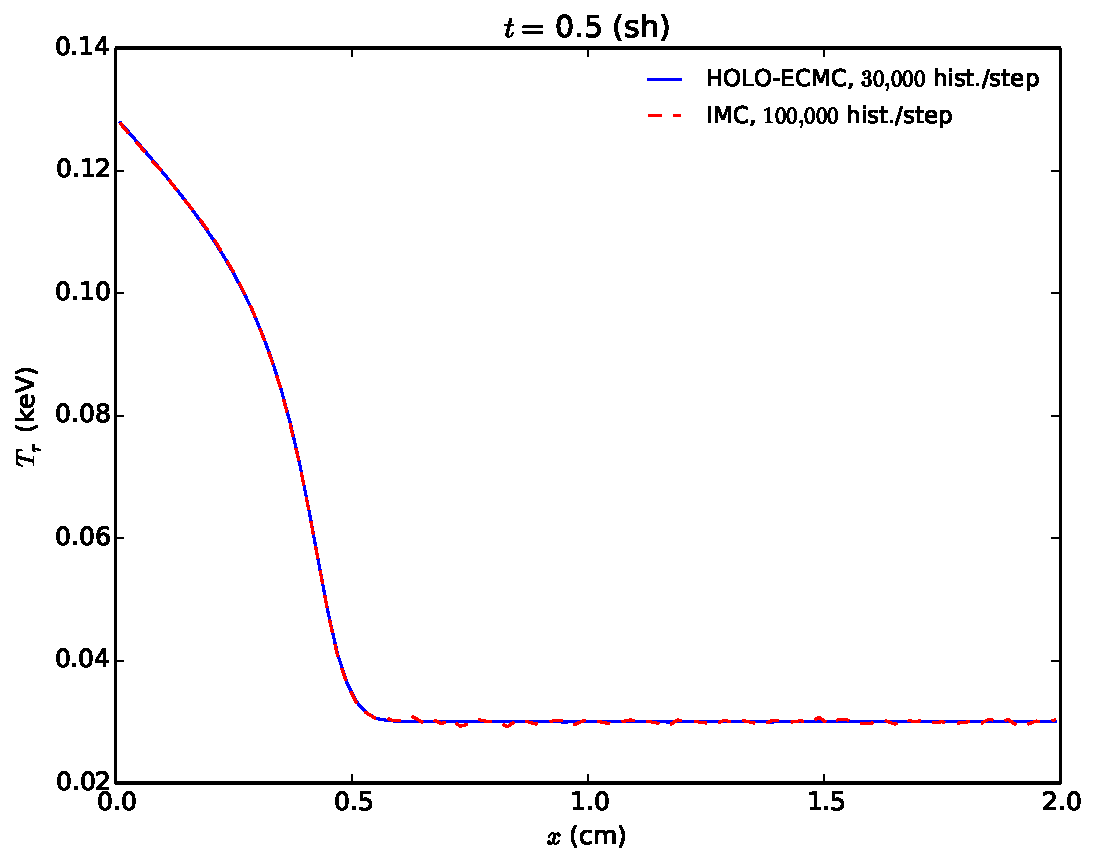
\includegraphics[width=0.65\textwidth]{heated_marshak.pdf}
    \caption{\label{hot_plot} Comparison of radiation temperatures for the pre-heated Marshak wave problem for 100
    $x$ cells at $\mathbf{t=0.5}$ sh.}
\end{figure}


\begin{table}[htbp]
\centering
\caption{\label{preheat_var} {Comparison of sample statistics for the 
    pre-heated marshak wave problem for 100 $x$ cells. Number of ECMC batches is
indicated in parenthesis.}}
\vspace{-0.1in}
\begin{tabular}{|c|ccc|ccc|}\cline{2-7}
    \multicolumn{1}{c|}{}       & \multicolumn{3}{|c|}{\ss} &
    \multicolumn{3}{|c|}{\FOM} \\ \hline
hists./step   & SMC & ECMC (1) & ECMC (3)  & SMC & ECMC (1) & ECMC (3)   \\ \hline
   12,000	  & 0.86\%   & 0.13\% & 0.24\% & 1      & 41  & 13      \\
  100,000     & 0.16\%   & 0.042\% & 0.08\% & 3.32   & 52  & 15       \\ 
  99,881 (AMR, 9 batches) & --  & \multicolumn{2}{c|}{ 0.038\%} & -- &
  \multicolumn{2}{c|}{61}               \\ \hline
\end{tabular}
\end{table}

\section{Accuracy in the Equilibrium Diffusion Limit}
\label{sec:edl_results}

As discussed in Sec.~\ref{sec:edl_overview}, we must ensure our method preserves the
equilibrium diffusion limit (EDL).
We have produced an EDL test problem by adjusting material properties to produce a strongly
diffusive domain. This EDL problem has constant cross sections with $\sigma_a=1000$
cm$^{-1}$, $\sigma_s=10$ cm$^{-1}$, $\rho c_v=6.8784\times 10^{-3}$ jk keV$^{-1}$
cm$^{-3}$.  The initial temperature is 0.01 keV and the domain width is 0.1 cm. The simulation
end time is 5 $sh$, and the step-size increases 5\% per time step from $\Delta t = 0.001$
sh to a maximum $\Delta t = 0.01$.
In all simulations, 4 $\mu$ cells and 3 batches of 4,000 histories were used for the
single HO solve, for each time step.
We compare HOLO results with a LDFE discretization and a step discretization of the LO
equations.  The step discretization, with a flat representation over each cell, is known
to be inaccurate in the EDL for S$_N$ equations.  The step discretization
is implemented with the step closure discussed in Sec.~\ref{sec:spat_clos_options} for all
cells.

The accuracy in the equilibrium diffusion limit is compared for the two spatial
discretizations, for different mesh sizes, in Fig.~\ref{fig:diff_limit}.  Visually, 
the LDFE spatial discretization has converged spatially, where both 20 and 200 cells
produce the same location of the wave front.  However, the step
discretization artificially propagates the energy forward, even for the 200 cells case; the inaccuracy is greater than
what would be expected from truncation error.  The step discretization will
only be accurate if the mesh cells are on the order of a mean free path, which is very large for this
problem.  Although not plotted, the material temperature overlays the radiation
temperature for the LDFE solution, in equilibrium with the radiation, as expected.
\begin{figure}[H]
    \centering
    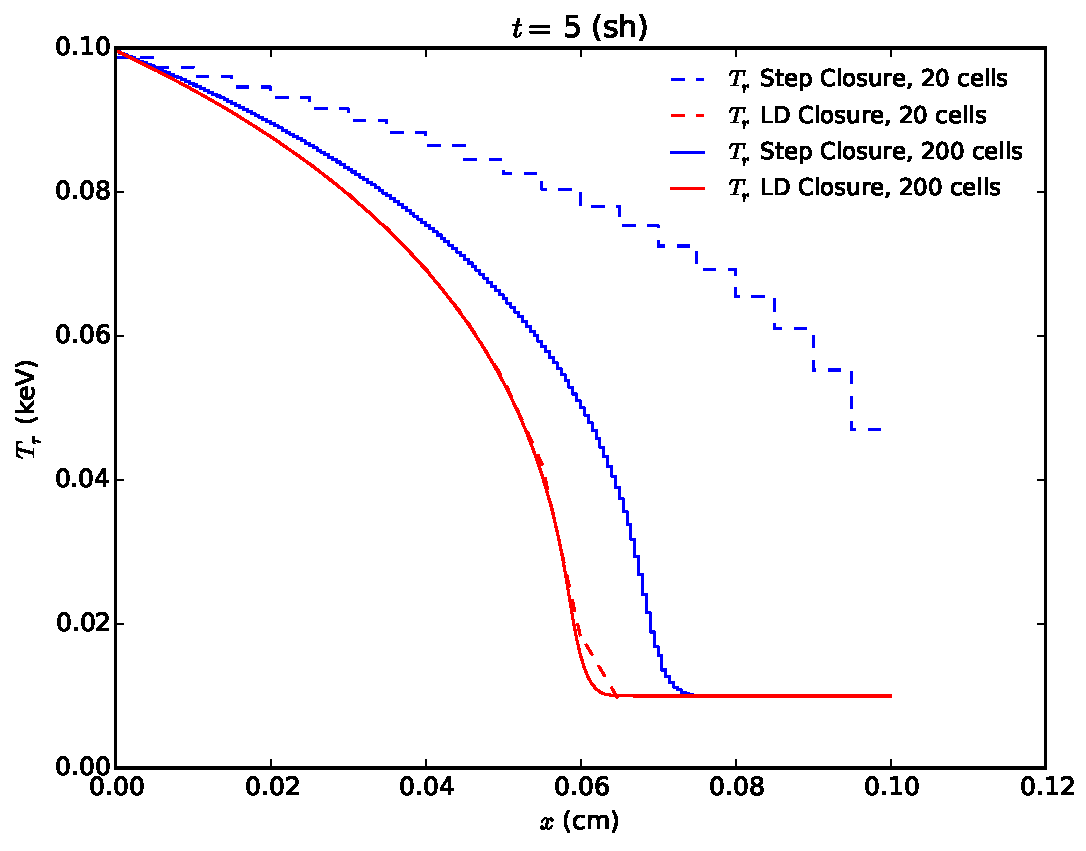
\includegraphics[width=0.6755799\textwidth]{diff_limit_compare.pdf}
    \caption{\label{fig:diff_limit}Comparison of $T_r$ for a problem in the equilibrium
    diffusion limit, with step and LDFE discretizations of the LO
equations.}
\end{figure}

\section{The HO Spatial Closure}

To investigate the utility of the face closures we compare to the LD spatial
closure for two test problems.  We are interested in the accuracy of the solution and
consistency between the HO and LO solutions, particularly for coarser meshes. 
The consistency for the $(l)$-th particular simulation is measured with the relative L$_2$ norm
of the difference between the projected HO and LO solutions, i.e.,
\begin{equation}
    \|\phi_{HO} - \phi_{LO}\|^{(l)}_{2,rel} = \frac{\ds \sqrt{\int_0^X \left(
        \phi_{HO}^{n+1,(l)}(x) - \phi_{LO}^{n+1,(l)}(x) \right)^2 \dd x}}{\ds \sqrt{
            \int_0^X \left(\phi_{LO}^{n+1,(l)}(x)\right)^2 \dd x }}
\end{equation}
where $\phi_{LO}(x)$ and $\phi_{HO}(x)$ are the LDFE representations in space of the
intensity from the HO and LO solvers, from the end of the last time step.
The error between a reference solution and a fine solution for the ${(l)}$-th simulation
is computed as
\begin{equation}
    \|e\|^{{(l)}}_{2,rel} = \frac{\|\phi_{LO}^{n+1,{(l)}}(x) -
    \phi_{LO}^{n+1,ref}\left( x \right)\|_2}{\|\phi_{LO}^{n+1,ref}\left( x \right)\|_2}
\end{equation}
All L$_2$ norms are computed using quadrature over the finest spatial mesh.  An
integrated measure of the error in cell-averaged mean intensities on the mesh of the
$l$-th simulation, with $N_c^{(l)}$ spatial cells, is computed as
\begin{equation}
    \|e\|^{{(l)}}_{a,rel} = \left({\frac{\ds \sum\limits_{i=1}^{N^{(l)}_c}
    \left(\phi_i^{n+1,{(l)}} - \phi_i^{n+1,ref}
\right)^2}{\ds \sum\limits_{i=1}^{N^{(l)}_c}\left(\phi_i^{n+1,ref}\right)^2}}\right)^{1/2},
\end{equation}
where $\phi_i^{n+1,ref}$ is computed by spatially averaging the fine mesh solution over
the $i$-th coarse spatial cell.

The sample mean of each of the above metrics is estimated based on 20 independent
simulations; the sample standard deviation for each \emph{mean} is also reported, e.g.,
\begin{equation}
    s\left(\|e\|_{2,rel}\right) = \left[\frac{1}{20-1}\sum_{l=1}^{20} \left(
    \|e\|_{2,rel}^{(l)} - \|e\|_{2,rel} \right)^2\right]^{1/2},
\end{equation}
where $\|e\|_{2,rel}=\sum_{l=1}^{20}\|e\|_{2,rel}^{(l)}/20$ is the mean.

\subsection{Smooth Problem}

For this problem, the radiation and material energies are initially in
equilibrium at $0.01$ keV.   An isotropic incident intensity of 0.05 keV is applied
at $x=0$; the incident intensity on the right boundary is $0.05$ keV.
The material properties are $\rho = 1$ g cm$^{-3}$, $c_v = 0.2$ jks/keV-g, and
$\sigma_a=10$ cm$^{-1}$.
The simulation end time is 0.5 sh.  The time step size increases by 10\% each time step
until the maximum step size of 0.01 sh is reached, beginning from $\Delta t = 0.001$ sh.
This problem is intended to have less steep gradients in the intensity by having constant constant cross
sections, a smaller boundary source, and diffusive problem parameters.
The problem has a smaller optical thickness than other problems tested so that the face-based solutions can be efficiently
estimated, but the small c$_v$ value makes the solution relatively diffusive.  This
problem did not require the lumped relation to produce positive solutions.
However, when projecting from a refined mesh back to the coarse mesh, it was
necessary to rotate the solution to be positive.

All simulations of this problem used 585,900 histories divided over 9 ECMC
batches;  beginning from 30,000 histories and $10$ $\mu$ cells, 30\% of cells were
adaptively refined every third batch, and the number of histories is increased to
keep the average number of histories per cell constant. 
We have have performed two outer HOLO iterations over each time step for all cases; it was
found that additional iterations did not increase consistency, because of the  magnitude
of statistical noise.  Relative convergence of HOLO iterations was below 10$^{-3}$
for two iterations for all cases.  
Fig.~\ref{fig:smooth_compare} compares cell-averaged radiation temperatures for various spatial closures at
coarse mesh sizes and a fine-mesh solution.  The HO spatial closures curve is for the
scaled-slope closure given by Eq.~\eqref{eq:cl_slope}.  There was visually
no difference in the results between the scaled-averaged, scaled-slope, or LD closure. A step closure in all cells
was inaccurate for this problem.

Table~\ref{tab:smooth} compares the different error metrics for different spatial
closures and numbers of cells.  The reference solution for all calculations was the average of 10 simulations with $N_c=500$ spatial
cells.  In all cases, the HO spatial closure produces higher accuracy in the L$_2$
norms and greater consistency between the solvers.  However, there is not an
improvement in accuracy of the cell-averaged intensities.  Neglecting noise, the LDFE representation can be third order
accurate for the $\|e\|_a$ norm and second-order accurate in the L$_2$ norm~\cite{morel_ldtrt}. 
The statistical noise induced in face tallies makes the
additional accuracy that the MC transport can use not greater than the benefit of
higher spatial integration by the MC transport.  It
is noted that, overall, there is very low statistical noise in each of these
solutions due to the ECMC method and relatively high number of histories; at lower
history counts, the small gains of the HO spatial closure will degrade and stability
becomes an issue.

\begin{figure}[H]
    \centering
    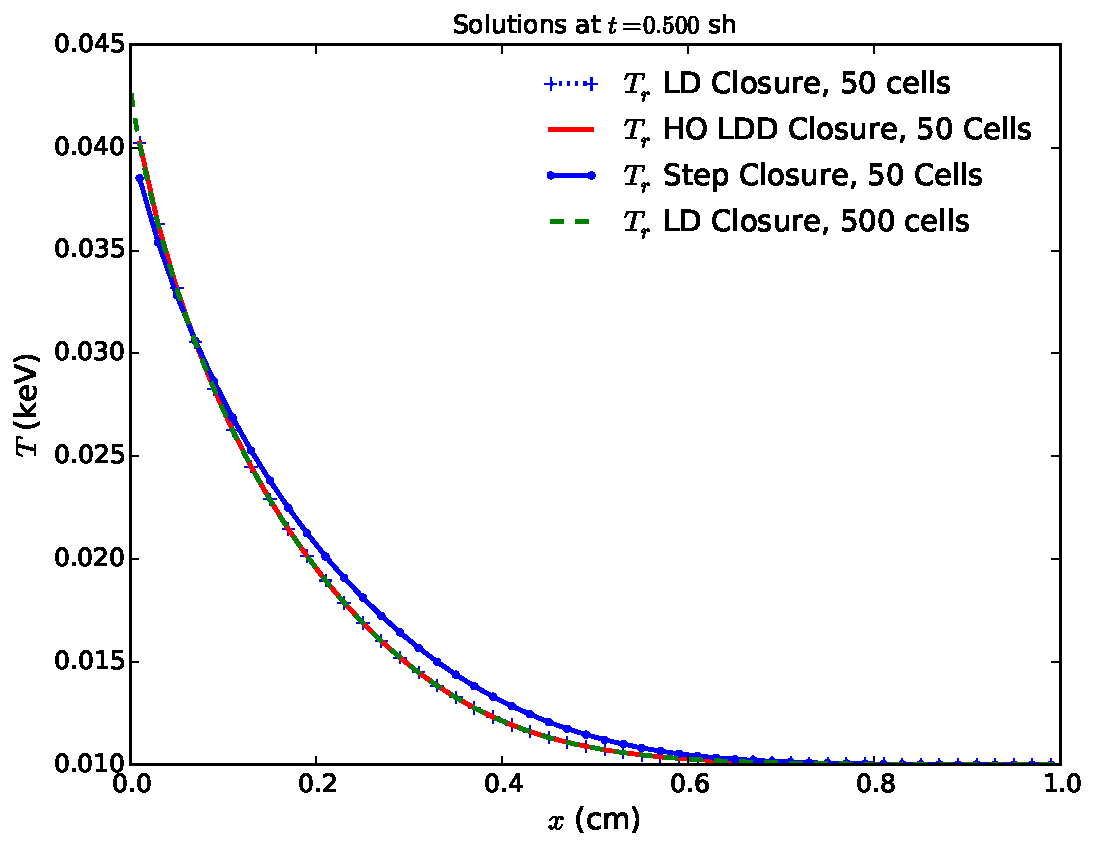
\includegraphics[width=0.99\linewidth]{smooth_compare.pdf}
    \caption{\label{fig:smooth_compare} Comparison of solutions for smooth problem with different spatial closures.}
\end{figure}

\begin{table}[H]
    \caption{\label{tab:smooth} Comparison of error metrics, reported as percentages, averaged over 20 simulations of smooth problem.  The absolute
standard deviation for each value is reported in parenthesis. Reference solution uses 500 cells.}
    \begin{tabular}{|l|cl|cl|cl|} \hline
        Spatial Closure & \multicolumn{2}{|c|}{$\|e\|_2$}  & \multicolumn{2}{|c|}{$\|e\|_{a}$} & \multicolumn{2}{|c|}{$\|\phi^{HO}
        -\phi^{LO}\|_{2}$} \\  \hline \hline
        \multicolumn{7}{|c|}{$N_c = 20$ cells} \\ \hline
LDFE               &   6.60\%  &   (0.17\%)  &   2.80\%     &   (5.7e-03\%)  &   2.90\%   &  (8.1e-03\%)  \\
HO: Scaled Slope   &   6.10\%  &   (2.9e-03\%)  &   3.50\%  &   (5.8e-03\%)  &   0.021\%  &  (8.6e-03\%)  \\
HO: Scaled Average &   6.10\%  &   (2.7e-03\%)  &   3.50\%  &   (5.0e-03\%)  &   0.023\%  &  (1.1e-02\%)  \\ \hline
       \multicolumn{7}{|c|}{$N_c  = 50$ cells}   \\ \hline
LDFE               &   1.60\%  &   (7.9e-04\%)  &   0.59\%  &   (3.8e-03\%)  &   0.76\%)  &  (4.8e-03\%)  \\
HO: Scaled Slope   &   1.40\%  &   (1.5e-03\%)  &   0.67\%  &   (3.2e-03\%)  &   0.012\%  &  (4.0e-03\%)  \\
HO: Scaled Average &   1.40\%  &   (1.5e-3\% ) &   0.67\%   &   (3.1e-03\%)  &   0.013\%  &  (3.9e-03\%)  \\ \hline
       \multicolumn{7}{|c|}{$N_c  = 100$ cells}   \\ \hline
LDFE               &   0.53\%  &   (2.1e-03\%)  &   0.15\%  &   (2.5e-03\%)  &   0.30\%)  &  (9.7e-03\%)  \%\\
HO: Scaled Slope   &   0.45\%  &   (1.5e-03\%)  &   0.16\%  &   (4.6e-03\%)  &   0.012\%  &  (4.8e-03\%)  \\
HO: Scaled Average &   0.45\%  &   (1.4e-03\%)  &   0.16\%  &   (4.7e-03\%)  &   0.012\%  &  (3.6e-03\%)  \\ \hline
    \end{tabular}
\end{table}



\subsection{Two Material Problem}

The HO spatial closures were applied to solution of the two material problem detailed in Sec.~\ref{sec:two}.
For these results, a small time step size of 0.001 sh was used, with a simulation end time
of 2 sh.  The scaled-slope closure was found to not stably converge, even for 2 batches of 10$^6$
histories.  The scale-average closure allowed for convergence, with the lumpded closure, but temperatures were driven
below the floor, and at times negative, leading to inaccurate solution.  The inaccuracies
result from the outflow being driving negative in cells near the wave front with steep
gradients.  The cause is that, although the HO solution was forced positive by scaling
moments, and the face solution is positive the closure does not necessarily agree with the
true moments. The first moment of the HO solution had to be modified to produce a positive
solution, and by trying to use the moment relation in the LO solution, there can be
negative solutions.  In general, in such difficult to resolve regions, the spatial closure
does not gain improvement.
Fig.~\ref{fig:two_mat_fail} depicts cell-averaged results at the end of the simulation.
The inaccuracy in ghtly overshoots, the slope changes signs between cells.  Additionally,
there is great inconsistency as the depressed temperature leads to an inaccurate HO solution.
A fundamental problem with the lumping relation is that the first moment equation for the
HO solution has a lumped temperature equation
\begin{figure}[H]
    \centering
    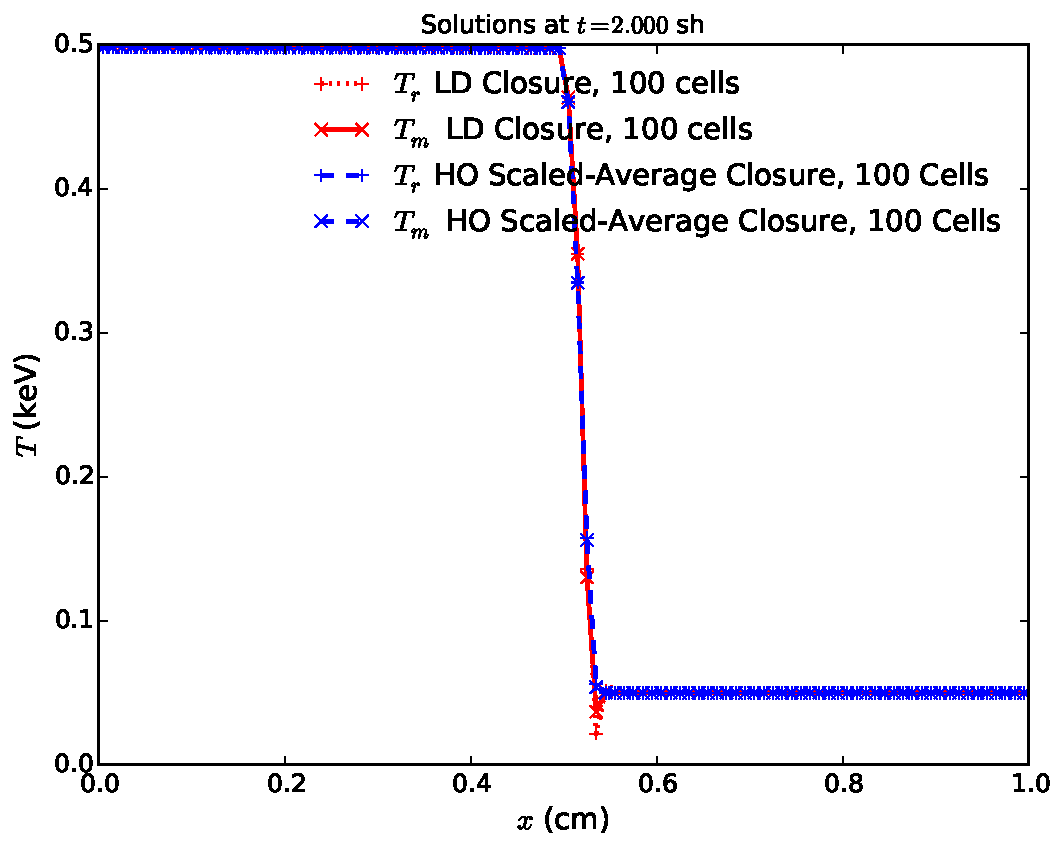
\includegraphics[width=0.6\linewidth]{two_mat_fail.pdf}
    %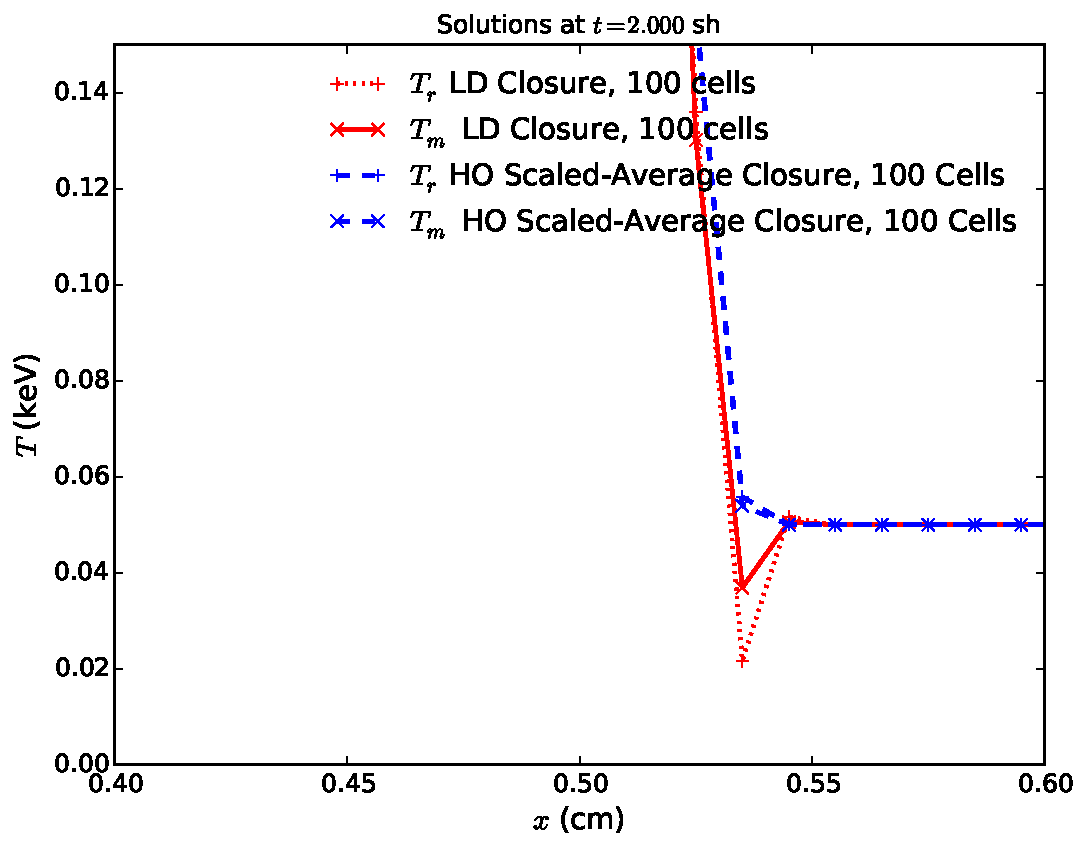
\includegraphics[width=0.99\linewidth]{two_mat_fail_zoom.pdf}
    \caption{\label{fig:two_mat_fail}Inacurracies for HO spatial closure applied to
    solution of the two material problem.}
\end{figure}




\section{Preservation of the Discrete Maximum Principle}

To numerically demonstrate that our method preserves the discrete MP, as discussed in
Sec.~\ref{sec:imc},  we have simulated problems similar to those
in~\cite{wollaber2013discrete}.  We produce a problem with tightly coupled
equations, by decreasing $c_v$ and increasing $\sigma_a$, which results in MP violations for IMC at various fixed time step sizes. 
The spatial and temporal discretization determine the occurrence of MP violations for
IMC. In particular, if time steps are too large or spatial
mesh cells are too small, IMC will demonstrate MP violations~\cite{wollaber2013discrete}.  Here, we have kept the
spatial mesh size fixed and increased the time step size to produce MP violations.
The material specifications are  $\sigma_{a} = \sigma_{a,0} T^{-3}$ cm$^{-1}$,
$\sigma_{a,0} = 4$ cm$^{-1}$ keV$^3$, $\sigma_s=0$ cm$^{-1}$, $\rho c_v = 0.0081181$
jks keV$^{-1}$ cm$^{-3}$.  The domain width is 2.0 cm with
$N_c=150$ uniform spatial mesh cells.  The radiation and material energies are initially in
equilibrium at $0.01$ keV, before an isotropic boundary source of $1$ keV is applied at
the left boundary at $t=0$. The simulation end time is $t=0.1$ sh. 

The material and radiation temperature are plotted for an IMC simulation with $\Delta
t=0.025$ sh in Figure~\ref{fig:imc_mpvrad}.  Figure~\ref{fig:imc_mpv} depicts the material temperature
for various time step sizes and the fixed mesh size of 150 cells. All IMC
simulations used 100,000 histories per time step. As demonstrated in
Fig.~\ref{fig:imc_mpvrad}, the material temperature exceeds the specified boundary
temperature and is artificially hotter than the radiation temperature.  This artificial
``temperature spike'' also leads to a slower propagation of the
wave~\cite{wollaber2013discrete}.  As shown in
Fig.~\ref{fig:imc_mpv}, as larger time-step sizes are taken the nonphysical results
worsen with the material temperature exceeding the radiation boundary temperature.
It is noted that although the final solution for $\Delta t=0.0001$ sh obeys the MP, during
the first few time steps the temperature spikes are present.
\begin{figure}[htbp]
    \centering
    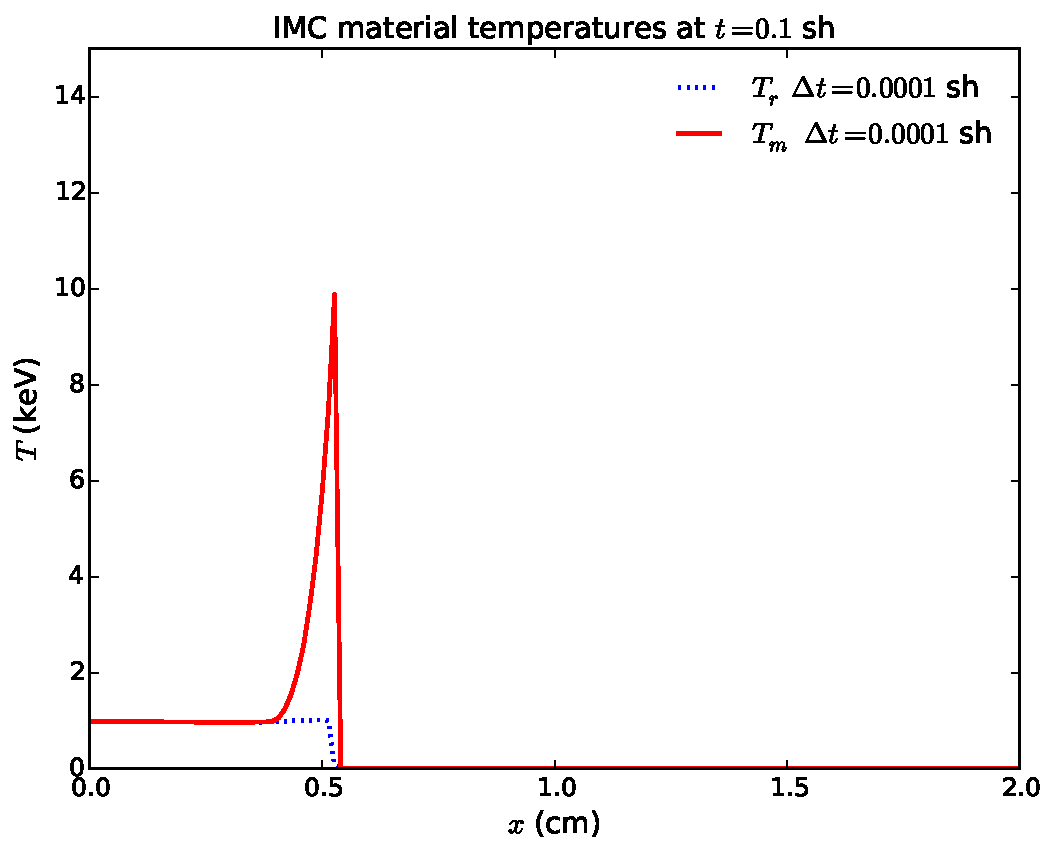
\includegraphics[width=0.6\linewidth]{mpv_rad_imc.pdf}
    \caption{\label{fig:imc_mpvrad}$T_r$ and $T$ for MP violation problem with IMC and $\Delta t = 0.001$ sh.}
\end{figure}
\begin{figure}[htbp]
    \centering
    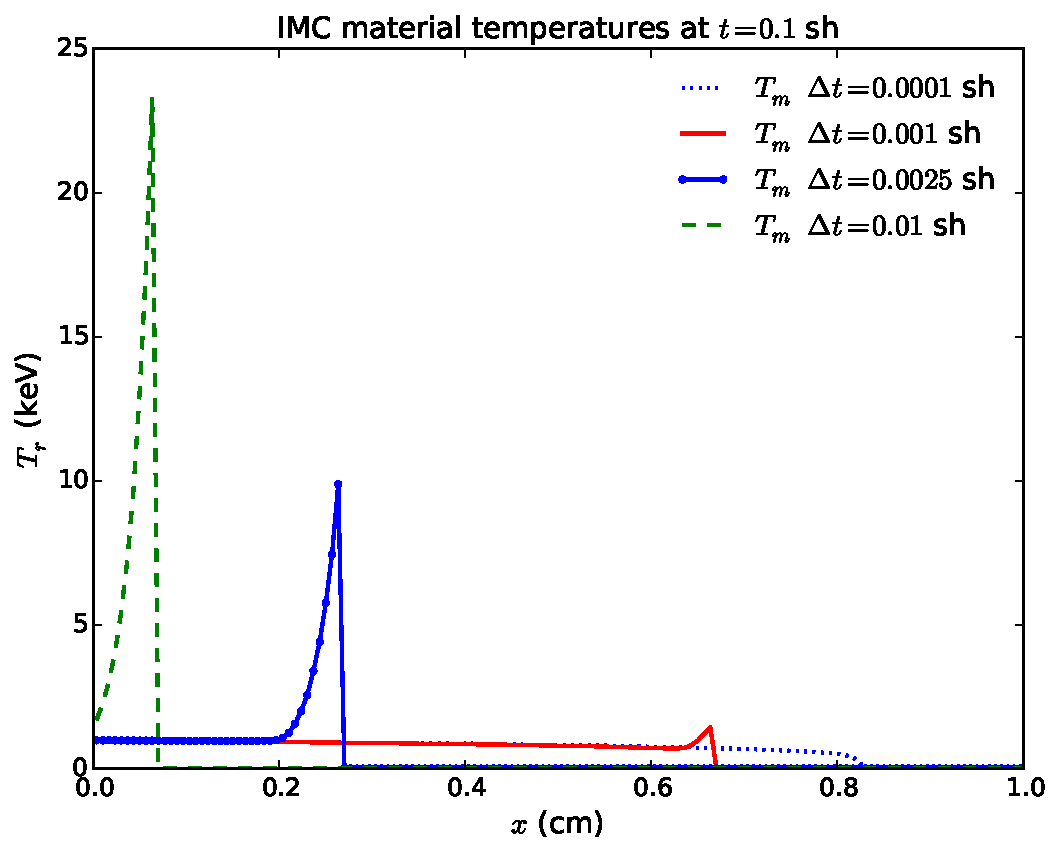
\includegraphics[width=0.6\linewidth]{mpv_mats_imc.pdf}
    \caption{\label{fig:imc_mpv}$T_m$ for MP violation problem with IMC for various time step
    sizes.}
\end{figure}

The simulations are repeated with the same specifications for the HOLO method. All HOLO
simulations used a fixed mesh of 8 $\mu$ cells by 150 $x$ cells, 3 batches per time step,
and 6,000 histories per batch. A single HO solve is performed per time step, and the LO
relative convergence tolerance is $10^{-6}$. The lumping closure is used for the radiation
terms in all spatial cells and any negativities in the HO solution are scaled to the floor
value as discussed in Sec.~\ref{sec:ho_easyfix}.  For these simulations, it was
necessary to use the damped Newton's method discussed in Sec.~\ref{sec:newton_overview} to converge the solutions~\cite{damped_newton}. 
 A fixed damping parameter with a factor of 0.5 was found to stably converge for all
 time-step sizes that were simulated. 

As seen in
Fig.~\ref{fig:holo_mpv}, the HOLO solution does not violate the maximum principle; the
temperature is bounded from above by the radiation boundary condition.
Table~\ref{tab:mpv_iters} demonstrates the LO Newton iteration counts for the HOLO method.
For reference, a solution with $\Delta t = 10^{-5}$ sh is given, which required no damping
to converge.  The damped iterations require more iterations to converge.  However, it is necessary to converge the nonlinear iterations to produce
physically meaningful solutions to this problem.  The advantage of the HOLO method is that
there is no additional cost for the HO solution when the damped method is used.
\begin{figure}[htbp]
    \centering
    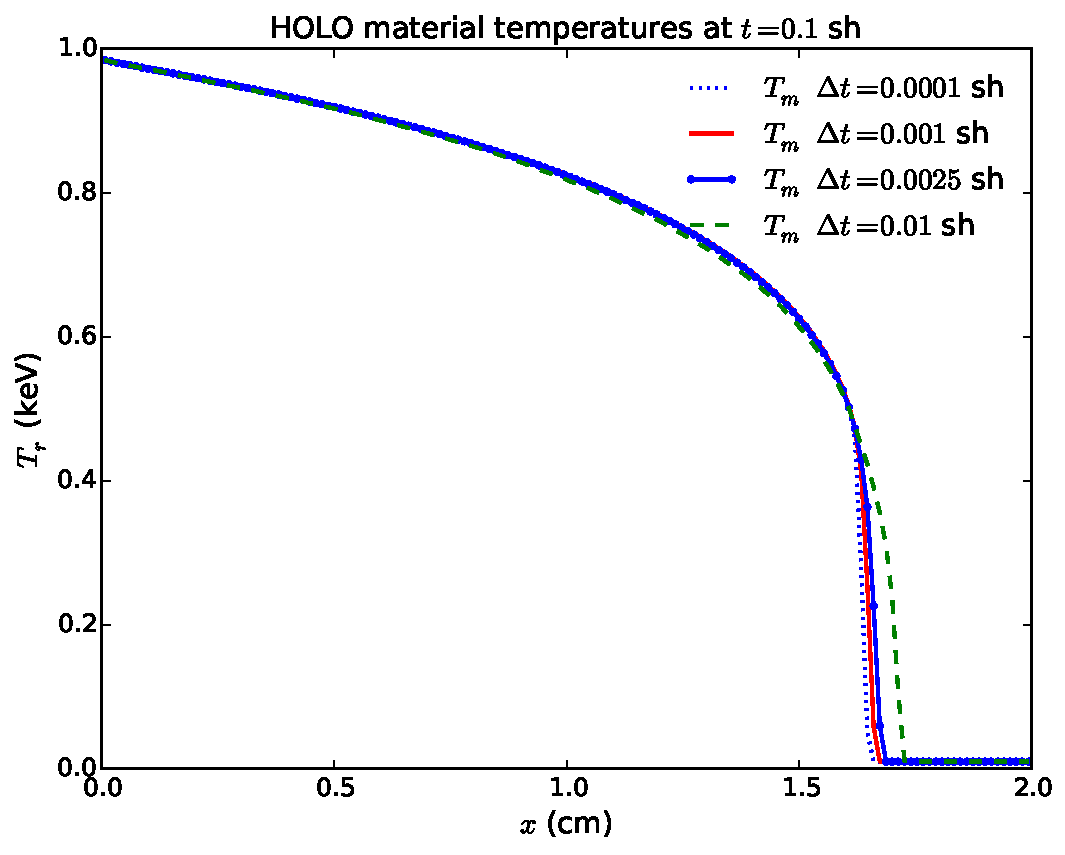
\includegraphics[width=0.6\linewidth]{mpv_mats_holo.pdf}
    \caption{\label{fig:holo_mpv}$T_m$ for MP violation problem with HOLO method for various time step
    sizes.}
\end{figure}
\begin{table}[htbp]
    \caption{\label{tab:mpv_iters}Comparison of LO Newton iterations for HOLO solution to 
    MP problem and different time step sizes. For $\Delta t=10^{-5}$ sh, no damping was used; for
    all other cases a damping factor of $0.5$ was used.}  
    \centering
        \begin{tabular}{|cc|} \hline
            $\Delta t$ (sh) & Newton Iters. / LO Solve \\ \hline
            $10^{-5}$    & 3.5 \\
            $10^{-4}$    & 21.0 \\
            $10^{-3}$    & 28.5 \\
            $2.5\times10^{-3}$  & 29.7 \\
            $10^{-2}$    & 46.3 \\ \hline
        \end{tabular}
\end{table}




